\chapter{Repository Remoti e Collaborazione}

\section*{Introduzione}
Git è un sistema distribuito: ogni clone è un repository completo. I repository remoti permettono collaborazione e backup centralizzato. Questo capitolo copre configurazione remote, sincronizzazione con clone/fetch/pull/push, e gestione di branch remoti.

\section*{Obiettivi di apprendimento}
\begin{itemize}
    \item Comprendere il concetto di repository remoto
    \item Configurare remote (\texttt{git remote})
    \item Clonare repository esistenti (\texttt{git clone})
    \item Sincronizzare modifiche (\texttt{fetch}, \texttt{pull}, \texttt{push})
    \item Gestire tracking branches
    \item Risolvere conflitti durante pull/push
    \item Best practices per collaborazione
    \item Gestire fork e upstream
\end{itemize}

\section{Concetto di Repository Remoto}

\subsection{Architettura distribuita}

In Git, ogni sviluppatore ha:
\begin{itemize}
    \item \textbf{Repository locale}: Copia completa con tutta la storia
    \item \textbf{Repository remoto}: Server centrale (GitHub, GitLab, BitBucket) per condivisione
\end{itemize}

\begin{figure}[h]
    \centering
    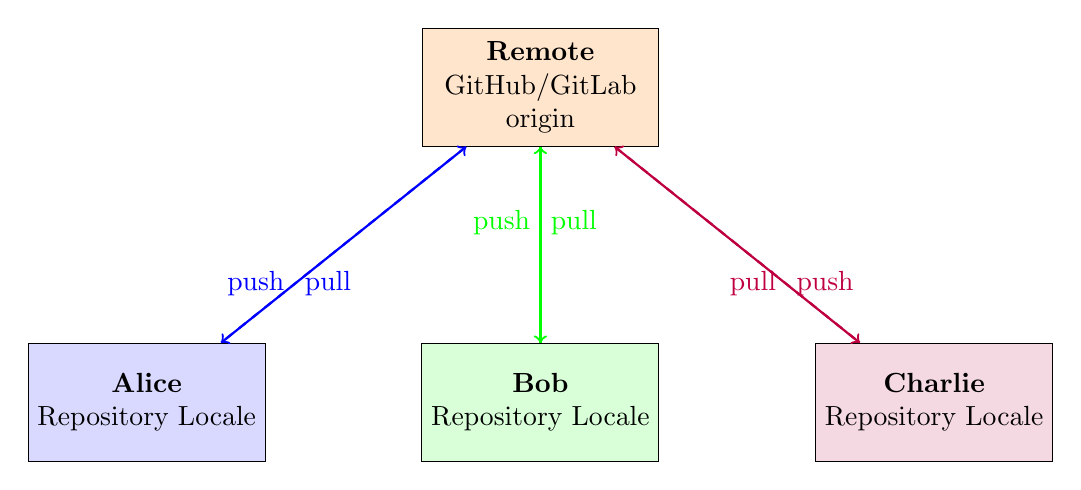
\begin{tikzpicture}[
        repo/.style={rectangle, draw, minimum width=2.5cm, minimum height=1.5cm, align=center},
        remote/.style={rectangle, draw, fill=orange!20, minimum width=3cm, minimum height=1.5cm, align=center},
        arrow/.style={->, thick}
    ]
        % Remote repository
        \node[remote] (remote) at (5,4) {
            \textbf{Remote}\\
            GitHub/GitLab\\
            origin
        };

        % Local repositories
        \node[repo, fill=blue!15] (alice) at (0,0) {
            \textbf{Alice}\\
            Repository Locale
        };

        \node[repo, fill=green!15] (bob) at (5,0) {
            \textbf{Bob}\\
            Repository Locale
        };

        \node[repo, fill=purple!15] (charlie) at (10,0) {
            \textbf{Charlie}\\
            Repository Locale
        };

        % Arrows
        \draw[arrow, blue] (alice) -- node[left, pos=0.3] {push} (remote);
        \draw[arrow, blue, dashed] (remote) -- node[right, pos=0.7] {pull} (alice);

        \draw[arrow, green] (bob) -- node[above left] {push} (remote);
        \draw[arrow, green, dashed] (remote) -- node[above right] {pull} (bob);

        \draw[arrow, purple] (charlie) -- node[right, pos=0.3] {push} (remote);
        \draw[arrow, purple, dashed] (remote) -- node[left, pos=0.7] {pull} (charlie);
    \end{tikzpicture}
    \caption{Architettura Git distribuita con remote centrale}
\end{figure}

\textbf{Workflow tipico}:
\begin{enumerate}
    \item \textbf{Clone}: Scarica repository da remote
    \item \textbf{Commit}: Lavora localmente, crea commit
    \item \textbf{Pull}: Scarica aggiornamenti da remote
    \item \textbf{Push}: Carica commit locali su remote
\end{enumerate}

\subsection{Vantaggi repository remoti}

\begin{tcolorbox}[colback=green!10, colframe=green!60, title=Vantaggi Remote Repository]
\begin{itemize}
    \item \textbf{Backup}: Codice salvato su server (disaster recovery)
    \item \textbf{Collaborazione}: Team condivide codice facilmente
    \item \textbf{Code review}: Pull request per review pre-merge
    \item \textbf{CI/CD}: Automazione test/deploy su push
    \item \textbf{Visibilità}: Storia progetto accessibile a tutti
    \item \textbf{Issue tracking}: GitHub Issues, GitLab Boards
    \item \textbf{Documentation}: Wiki, README, GitHub Pages
\end{itemize}
\end{tcolorbox}

\section{Gestire Remote: git remote}

\subsection{Visualizzare remote configurati}

\begin{lstlisting}[caption=Listare remote]
# Lista remote (solo nomi)
$ git remote
origin

# Lista remote con URL
$ git remote -v
origin  https://github.com/user/repo.git (fetch)
origin  https://github.com/user/repo.git (push)

# Dettagli remote specifico
$ git remote show origin
* remote origin
  Fetch URL: https://github.com/user/repo.git
  Push  URL: https://github.com/user/repo.git
  HEAD branch: main
  Remote branches:
    main    tracked
    develop tracked
  Local branch configured for 'git pull':
    main merges with remote main
  Local ref configured for 'git push':
    main pushes to main (up to date)
\end{lstlisting}

\subsection{Aggiungere remote}

\begin{lstlisting}[caption=Aggiungere remote repository]
# Aggiungi remote chiamato "origin"
$ git remote add origin https://github.com/user/repo.git

# Verifica aggiunta
$ git remote -v
origin  https://github.com/user/repo.git (fetch)
origin  https://github.com/user/repo.git (push)

# Aggiungi secondo remote (es: fork upstream)
$ git remote add upstream https://github.com/original/repo.git

$ git remote -v
origin    https://github.com/user/repo.git (fetch)
origin    https://github.com/user/repo.git (push)
upstream  https://github.com/original/repo.git (fetch)
upstream  https://github.com/original/repo.git (push)
\end{lstlisting}

\textbf{Convenzioni naming}:
\begin{itemize}
    \item \textbf{origin}: Remote principale (tuo repository)
    \item \textbf{upstream}: Repository originale (in caso di fork)
    \item Nomi custom: staging, production, backup, etc.
\end{itemize}

\subsection{Modificare e rimuovere remote}

\begin{lstlisting}[caption=Gestione remote]
# Rinomina remote
$ git remote rename origin upstream
$ git remote
upstream

# Cambia URL remote
$ git remote set-url origin https://github.com/newuser/repo.git

# Cambia URL da HTTPS a SSH
$ git remote set-url origin git@github.com:user/repo.git

# Rimuovi remote
$ git remote remove upstream
$ git remote
origin
\end{lstlisting}

\subsection{HTTPS vs SSH}

\textbf{HTTPS}:
\begin{lstlisting}
https://github.com/user/repo.git
\end{lstlisting}

\textbf{Pros}: Setup semplice, funziona ovunque\\
\textbf{Cons}: Richiede username/password (o token) ogni push

\textbf{SSH}:
\begin{lstlisting}
git@github.com:user/repo.git
\end{lstlisting}

\textbf{Pros}: Autenticazione automatica con SSH keys, più sicuro\\
\textbf{Cons}: Richiede setup chiavi SSH

\begin{tcolorbox}[colback=green!10, colframe=green!60, title=Best Practice: Usa SSH]
Per repository frequenti, configura SSH keys. Eviti di inserire credenziali ogni volta:

\begin{verbatim}
# Genera SSH key
$ ssh-keygen -t ed25519 -C "your_email@example.com"

# Aggiungi key a ssh-agent
$ ssh-add ~/.ssh/id_ed25519

# Copia public key e aggiungila su GitHub Settings > SSH Keys
$ cat ~/.ssh/id_ed25519.pub
\end{verbatim}
\end{tcolorbox}

\section{Clonare Repository: git clone}

\subsection{Clone base}

\begin{lstlisting}[caption=Clonare repository]
# Clone da GitHub
$ git clone https://github.com/user/repo.git
Cloning into 'repo'...
remote: Enumerating objects: 3, done.
remote: Counting objects: 100% (3/3), done.
remote: Total 3 (delta 0), reused 0 (delta 0)
Receiving objects: 100% (3/3), done.

$ cd repo
$ git remote -v
origin  https://github.com/user/repo.git (fetch)
origin  https://github.com/user/repo.git (push)
\end{lstlisting}

\textbf{Cosa fa \texttt{git clone}}:
\begin{enumerate}
    \item Crea directory con nome del repository
    \item Inizializza \texttt{.git/}
    \item Configura \texttt{origin} remote
    \item Scarica tutta la storia
    \item Checkout branch default (main/master)
    \item Configura tracking per branch default
\end{enumerate}

\subsection{Opzioni clone}

\begin{lstlisting}[caption=Clone con opzioni]
# Clone con nome directory custom
$ git clone https://github.com/user/repo.git mio-progetto

# Shallow clone (solo ultimo commit, risparmia spazio)
$ git clone --depth 1 https://github.com/user/repo.git

# Clone singolo branch
$ git clone --branch develop --single-branch https://github.com/user/repo.git

# Clone bare (senza working directory, per server)
$ git clone --bare https://github.com/user/repo.git repo.git
\end{lstlisting}

\textbf{Shallow clone use cases}:
\begin{itemize}
    \item CI/CD: Build solo ultimo stato
    \item Download veloce di repo enormi
    \item Demo/testing rapido
\end{itemize}

\textbf{Limitazioni shallow clone}:
\begin{itemize}
    \item Non puoi push
    \item Git log limitato
    \item Alcuni comandi non funzionano
\end{itemize}

\section{Fetch: Scaricare Aggiornamenti}

\subsection{Concetto di fetch}

\texttt{git fetch} scarica commit da remote \textbf{senza} modificare working directory. Aggiorna solo remote-tracking branches.

\begin{figure}[h]
    \centering
    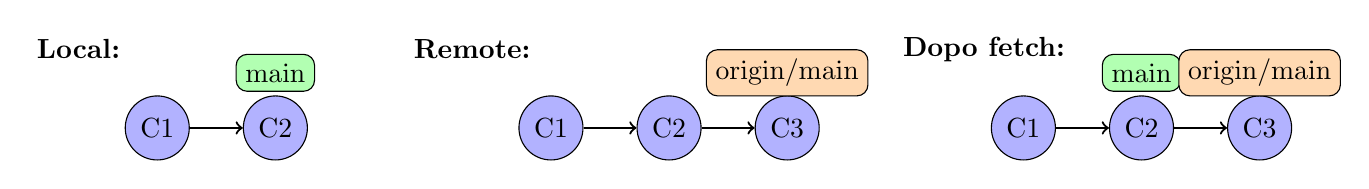
\begin{tikzpicture}[
        commit/.style={circle, draw, fill=blue!30, minimum size=0.7cm},
        branch/.style={rectangle, draw, fill=green!30, rounded corners},
        arrow/.style={->, thick}
    ]
        % Local
        \node at (-1, 2) {\textbf{Local:}};
        \node[commit] (c1) at (0,1) {C1};
        \node[commit] (c2) at (1.5,1) {C2};
        \node[branch] (main) at (1.5,1.7) {main};

        \draw[arrow] (c1) -- (c2);

        % Remote
        \node at (4, 2) {\textbf{Remote:}};
        \node[commit] (c1r) at (5,1) {C1};
        \node[commit] (c2r) at (6.5,1) {C2};
        \node[commit] (c3r) at (8,1) {C3};
        \node[branch, fill=orange!30] (origin) at (8,1.7) {origin/main};

        \draw[arrow] (c1r) -- (c2r);
        \draw[arrow] (c2r) -- (c3r);

        % After fetch
        \node at (10.5, 2) {\textbf{Dopo fetch:}};
        \node[commit] (c1f) at (11,1) {C1};
        \node[commit] (c2f) at (12.5,1) {C2};
        \node[commit] (c3f) at (14,1) {C3};
        \node[branch] (mainf) at (12.5,1.7) {main};
        \node[branch, fill=orange!30] (originf) at (14,1.7) {origin/main};

        \draw[arrow] (c1f) -- (c2f);
        \draw[arrow] (c2f) -- (c3f);
    \end{tikzpicture}
    \caption{Fetch aggiorna origin/main, main rimane invariato}
\end{figure}

\begin{lstlisting}[caption=git fetch esempi]
# Fetch da origin (default remote)
$ git fetch
remote: Enumerating objects: 5, done.
remote: Counting objects: 100% (5/5), done.
Receiving objects: 100% (3/3), done.

# Fetch da remote specifico
$ git fetch upstream

# Fetch tutti i remote
$ git fetch --all

# Fetch e prune branch remoti eliminati
$ git fetch --prune
\end{lstlisting}

\subsection{Visualizzare branch remoti}

\begin{lstlisting}[caption=Branch remoti dopo fetch]
# Lista branch remote
$ git branch -r
  origin/main
  origin/develop
  origin/feature/login

# Lista tutti (locali + remoti)
$ git branch -a
* main
  develop
  remotes/origin/main
  remotes/origin/develop
  remotes/origin/feature/login

# Log branch remoto
$ git log origin/main

# Confronta local vs remote
$ git log main..origin/main  # Commit in remote non in local
$ git log origin/main..main  # Commit in local non in remote
\end{lstlisting}

\section{Pull: Scaricare e Merge}

\subsection{git pull = fetch + merge}

\texttt{git pull} combina \texttt{fetch} e \texttt{merge}:

\begin{lstlisting}[caption=git pull]
# Pull = fetch + merge
$ git pull
# Equivalente a:
$ git fetch origin
$ git merge origin/main

# Pull da remote/branch specifici
$ git pull origin develop

# Pull con rebase invece di merge
$ git pull --rebase
# Equivalente a:
$ git fetch origin
$ git rebase origin/main
\end{lstlisting}

\begin{tcolorbox}[colback=orange!10, colframe=orange!60, title=Nota: Pull Default Behavior]
\texttt{git pull} senza argomenti:
\begin{itemize}
    \item Usa remote configurato per branch corrente (di solito \texttt{origin})
    \item Mergia tracking branch corrispondente
    \item Se non configurato, richiede specificare remote/branch
\end{itemize}
\end{tcolorbox}

\subsection{Pull con conflitti}

\begin{lstlisting}[caption=Risolvere conflitti durante pull]
$ git pull
Auto-merging main.py
CONFLICT (content): Merge conflict in main.py
Automatic merge failed; fix conflicts and then commit the result.

# Risolvi conflitti manualmente
$ vim main.py

# Stage file risolto
$ git add main.py

# Completa merge
$ git commit
[main a4b6c8d] Merge branch 'main' of https://github.com/user/repo

# Oppure abbandona pull
$ git merge --abort
\end{lstlisting}

\subsection{Pull rebase}

\begin{lstlisting}[caption=Pull con rebase per storia lineare]
# Pull con rebase
$ git pull --rebase

# Configura rebase come default per pull
$ git config --global pull.rebase true

# Storia lineare senza merge commit
$ git log --oneline --graph
* c3 (HEAD -> main, origin/main) Remote commit
* c2 Your local commit
* c1 Initial commit
\end{lstlisting}

\begin{tcolorbox}[colback=green!10, colframe=green!60, title=Best Practice: Pull Rebase]
\texttt{git pull --rebase} è preferibile per storia pulita:
\begin{itemize}
    \item Evita merge commit inutili
    \item Storia lineare e leggibile
    \item Commit locali "sopra" commit remoti
\end{itemize}

Usa solo se:
\begin{itemize}
    \item Commit locali non ancora pushati
    \item Storia locale non condivisa
\end{itemize}
\end{tcolorbox}

\section{Push: Caricare Commit}

\subsection{Push base}

\begin{lstlisting}[caption=Pushare commit su remote]
# Push branch corrente su origin
$ git push
Enumerating objects: 3, done.
Counting objects: 100% (3/3), done.
Writing objects: 100% (3/3), 280 bytes | 280.00 KiB/s, done.
Total 3 (delta 0), reused 0 (delta 0)
To https://github.com/user/repo.git
   a3f5b21..b8c9d34  main -> main

# Push specificando remote e branch
$ git push origin main

# Push e imposta tracking
$ git push -u origin feature/nuova
# Equivalente a:
$ git push --set-upstream origin feature/nuova
\end{lstlisting}

\textbf{Cosa fa \texttt{-u}/\texttt{--set-upstream}}:
\begin{itemize}
    \item Crea branch remoto se non esiste
    \item Configura tracking tra branch locale e remoto
    \item Successivi \texttt{git push} non richiedono argomenti
\end{itemize}

\subsection{Push tutti i branch}

\begin{lstlisting}[caption=Push multipli branch]
# Push tutti i branch
$ git push --all

# Push anche tag
$ git push --tags

# Push tutto (branch + tag)
$ git push --all && git push --tags
\end{lstlisting}

\subsection{Push rejected}

\begin{lstlisting}[caption=Push rifiutato - remote ha commit nuovi]
$ git push
To https://github.com/user/repo.git
 ! [rejected]        main -> main (fetch first)
error: failed to push some refs to 'https://github.com/user/repo.git'
hint: Updates were rejected because the remote contains work that you do
hint: not have locally. This is usually caused by another repository pushing
hint: to the same ref. You may want to first integrate the remote changes
hint: (e.g., 'git pull ...') before pushing again.
\end{lstlisting}

\textbf{Soluzione}:
\begin{lstlisting}[caption=Integrare modifiche remote prima di push]
# Pull modifiche remote (fetch + merge)
$ git pull

# Risolvi eventuali conflitti

# Riprova push
$ git push
\end{lstlisting}

\subsection{Force push}

\begin{lstlisting}[caption=Force push - PERICOLOSO]
# Force push (sovrascrive remote)
$ git push --force
# Equivalente (più safe):
$ git push --force-with-lease
\end{lstlisting}

\begin{tcolorbox}[colback=red!10, colframe=red!60, title=ATTENZIONE: Force Push]
\texttt{git push --force} sovrascrive storia remota. \textbf{Estremamente pericoloso} su branch condivisi:

\textbf{Quando è OK}:
\begin{itemize}
    \item Branch privato personale
    \item Dopo rebase interattivo su feature branch
    \item Fix commit message su branch non condiviso
\end{itemize}

\textbf{Quando NON usare}:
\begin{itemize}
    \item Mai su \texttt{main}/\texttt{master}
    \item Mai su branch condivisi con altri
    \item Mai se non sai cosa stai facendo
\end{itemize}

\textbf{Alternativa più safe}: \texttt{--force-with-lease} (fallisce se remote ha commit non previsti)
\end{tcolorbox}

\subsection{Eliminare branch remoto}

\begin{lstlisting}[caption=Eliminare branch su remote]
# Elimina branch remoto
$ git push origin --delete feature/vecchia
To https://github.com/user/repo.git
 - [deleted]         feature/vecchia

# Metodo alternativo (push "nothing" al branch)
$ git push origin :feature/vecchia
\end{lstlisting}

\section{Tracking Branches}

\subsection{Cosa sono tracking branches}

\textbf{Tracking branch}: Branch locale configurato per seguire branch remoto.

\begin{lstlisting}[caption=Configurare tracking]
# Crea branch locale trackando remoto
$ git checkout -b feature origin/feature
Branch 'feature' set up to track remote branch 'feature' from 'origin'.
Switched to a new branch 'feature'

# Metodo moderno (Git 2.23+)
$ git switch -c feature origin/feature

# Imposta tracking su branch esistente
$ git branch --set-upstream-to=origin/main main
Branch 'main' set up to track remote branch 'main' from 'origin'.

# Abbreviazione
$ git branch -u origin/main main
\end{lstlisting}

\subsection{Visualizzare tracking}

\begin{lstlisting}[caption=Vedere configurazione tracking]
# Branch con tracking info
$ git branch -vv
* main    a3f5b21 [origin/main: ahead 2, behind 1] Latest commit
  develop b8c9d34 [origin/develop] Develop work
  feature c7e2a19 Not tracking anything

# Spiegazione:
# ahead 2  = 2 commit locali non pushati
# behind 1 = 1 commit remoto non pullato
\end{lstlisting}

\subsection{Vantaggi tracking branches}

\begin{itemize}
    \item \texttt{git pull} senza argomenti (sa da dove pullare)
    \item \texttt{git push} senza argomenti (sa dove pushare)
    \item \texttt{git status} mostra ahead/behind
    \item Comandi più concisi
\end{itemize}

\section{Fork e Upstream}

\subsection{Workflow con fork}

Contribuire a progetti open source:

\begin{enumerate}
    \item \textbf{Fork}: Crea copia del repo su tuo account GitHub
    \item \textbf{Clone}: Clona tuo fork localmente
    \item \textbf{Add upstream}: Aggiungi repo originale come remote
    \item \textbf{Branch}: Crea feature branch
    \item \textbf{Commit}: Sviluppa feature
    \item \textbf{Push}: Push su tuo fork
    \item \textbf{Pull Request}: Proponi merge a repo originale
\end{enumerate}

\begin{lstlisting}[caption=Setup fork workflow]
# 1. Fork su GitHub (click button "Fork")

# 2. Clone tuo fork
$ git clone https://github.com/tuousername/progetto.git
$ cd progetto

# 3. Aggiungi upstream (repo originale)
$ git remote add upstream https://github.com/originale/progetto.git

# 4. Verifica remote
$ git remote -v
origin    https://github.com/tuousername/progetto.git (fetch)
origin    https://github.com/tuousername/progetto.git (push)
upstream  https://github.com/originale/progetto.git (fetch)
upstream  https://github.com/originale/progetto.git (push)
\end{lstlisting}

\subsection{Sync fork con upstream}

\begin{lstlisting}[caption=Aggiornare fork da upstream]
# Fetch modifiche da upstream
$ git fetch upstream

# Merge upstream/main in tuo main
$ git checkout main
$ git merge upstream/main

# Push modifiche su tuo fork
$ git push origin main

# Workflow completo in un comando (con rebase)
$ git pull upstream main --rebase
$ git push origin main
\end{lstlisting}

\section*{Riepilogo concetti chiave}

\begin{tcolorbox}[colback=gray!10, colframe=black!60, title=Concetti fondamentali]
\begin{itemize}
    \item \textbf{Remote}: Repository su server (GitHub, GitLab) per condivisione
    \item \texttt{git remote add} configura remote, convenzione: \texttt{origin}
    \item \texttt{git clone} scarica repository completo e configura origin
    \item \texttt{git fetch} scarica commit senza modificare working directory
    \item \texttt{git pull} = fetch + merge (o rebase con \texttt{--rebase})
    \item \texttt{git push} carica commit locali su remote
    \item \texttt{-u}/\texttt{--set-upstream} configura tracking branch
    \item \textbf{Tracking branch}: Branch locale associato a remote
    \item \textbf{Fork workflow}: fork → clone → upstream → feature → PR
    \item \texttt{--force} è pericoloso, usa solo su branch privati
\end{itemize}
\end{tcolorbox}

\section*{Esercizi}

\begin{enumerate}
    \item Crea repository su GitHub, clonalo localmente, verifica remote con \texttt{git remote -v}.

    \item Aggiungi file, committi, pusha su remote con \texttt{git push -u origin main}.

    \item Modifica file su GitHub web, usa \texttt{git fetch} poi \texttt{git merge origin/main} separatamente.

    \item Pratica \texttt{git pull --rebase} per storia lineare.

    \item Crea branch locale, pusha con \texttt{-u}, poi usa \texttt{git push} senza argomenti.

    \item Simula conflitto: modifica stessa riga localmente e su remote, risolvi durante pull.

    \item Configura SSH key per GitHub, cambia remote da HTTPS a SSH.

    \item Fork repository open source, aggiungi upstream, sync fork.

    \item Usa \texttt{git branch -vv} per vedere ahead/behind status.

    \item Crea shallow clone con \texttt{--depth 1}, confronta dimensione con clone normale.
\end{enumerate}

\section*{Riferimenti}

\begin{itemize}
    \item Git Remote: \url{https://git-scm.com/book/en/v2/Git-Basics-Working-with-Remotes}
    \item GitHub SSH Setup: \url{https://docs.github.com/en/authentication/connecting-to-github-with-ssh}
    \item Fork workflow: \url{https://docs.github.com/en/get-started/quickstart/fork-a-repo}
\end{itemize}
